% !Mode:: "TeX:UTF-8"
% !TEX program  = xelatex
\section{Analysis of model structure and parameter setting}
\subsection{Performance of Autoencoder, VAE and ZIVA}
Our model was adapted from the variational autoencoder (VAE). The major improvement is the zero-inflation layer. So, I analyzed the significance of ZI layer in this part. I performed the Autoencoder, Variational autoencoder and ZIVA to several data and evaluated their performance on visualization and clustering. We performed visualization (Figure \ref{3ae}) and clustering (Table \ref{nmi3ae} and \ref{ari3ae} ,Figure \ref{3aeclu}) to the dimensionality reduction results under two dimensions. Both of the visualization and the clustering evaluation show that ZIVA has better performance than autoencoder and variational autoencoder. It is proven that the zero-inflation layer works in our network structure. \\
\begin{figure}[htb!]
    \centering
    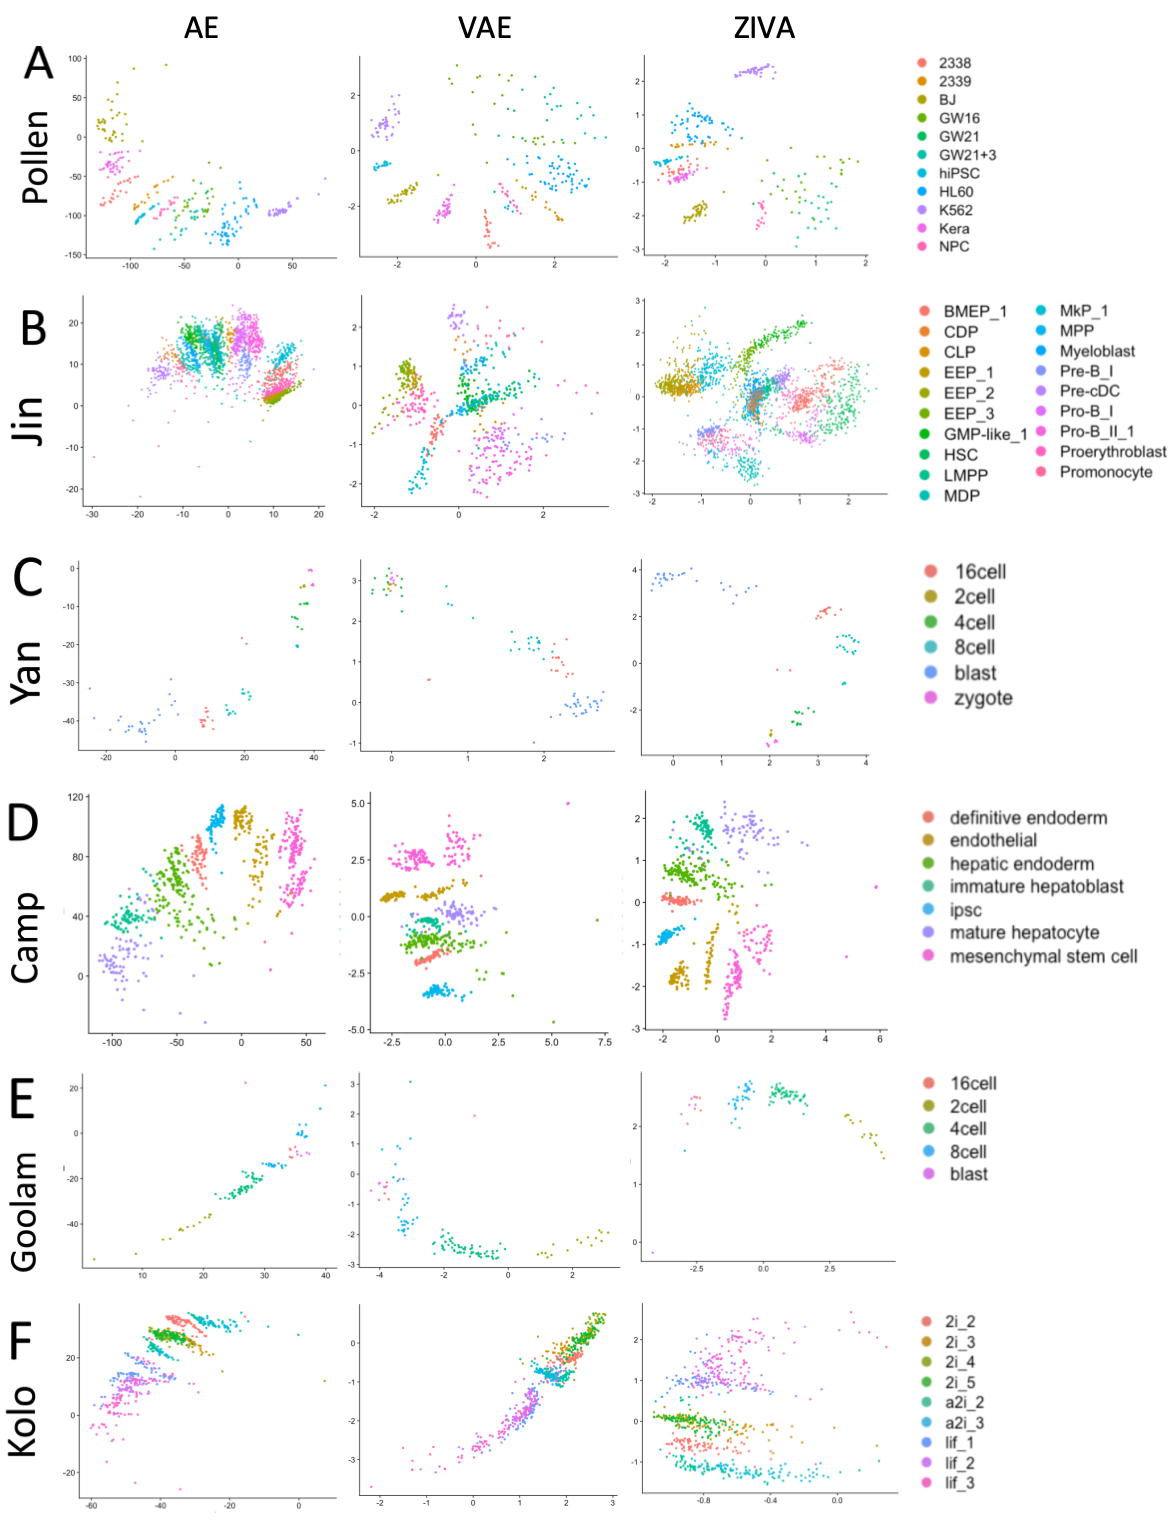
\includegraphics[width=0.8\textwidth]{figures/myfigures/3ae.png}
    \caption{Visualization of scRNA-seq datasets using Autoencoder, Variational autoencoder (VAE) and ZIVA}
    \label{3ae}
\end{figure}
\begin{figure}[htb!]
    \centering
    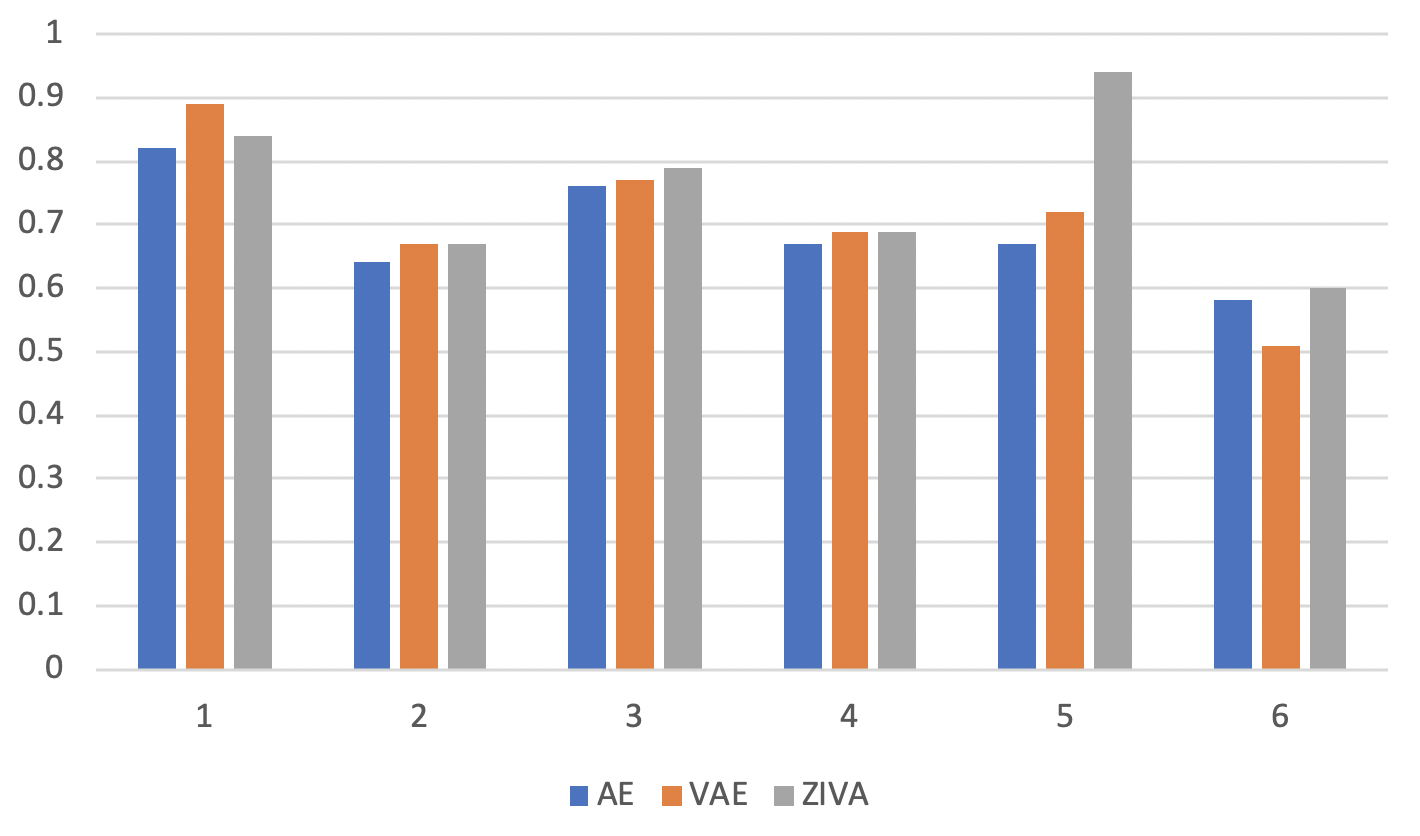
\includegraphics[width=0.8\textwidth]{figures/myfigures/3aeclu.png}
    \caption{Clustering performance comparation among Autoencoder, Variational autoencoder (VAE) and ZIVA}
    \label{3aeclu}
\end{figure}
\subsection{Analysis of dropout model}
Then, we tested the performance of two dropout models: the negative binomial model and the Michaelis-Menten model. We tested the performance of clustering on the data reduced to two dimensions by two methods. The result (Table 7) shows that two model have similar performance on those datasets.



\subsection{Analysis of latent dimensions}
Then, I tested the clustering performance under different latent dimensions (2, 4, 6, 8, 10, 15, 20, all). The result (Table \ref{dimt}, Figure \ref{dim}) shows that there is no significance difference among different latent dimensions. The performance on 2 dimensions and all dimensions are slightly higher. According to this result, the first two dimension is enough downstream analysis.
\begin{figure}[htb!]
    \centering
    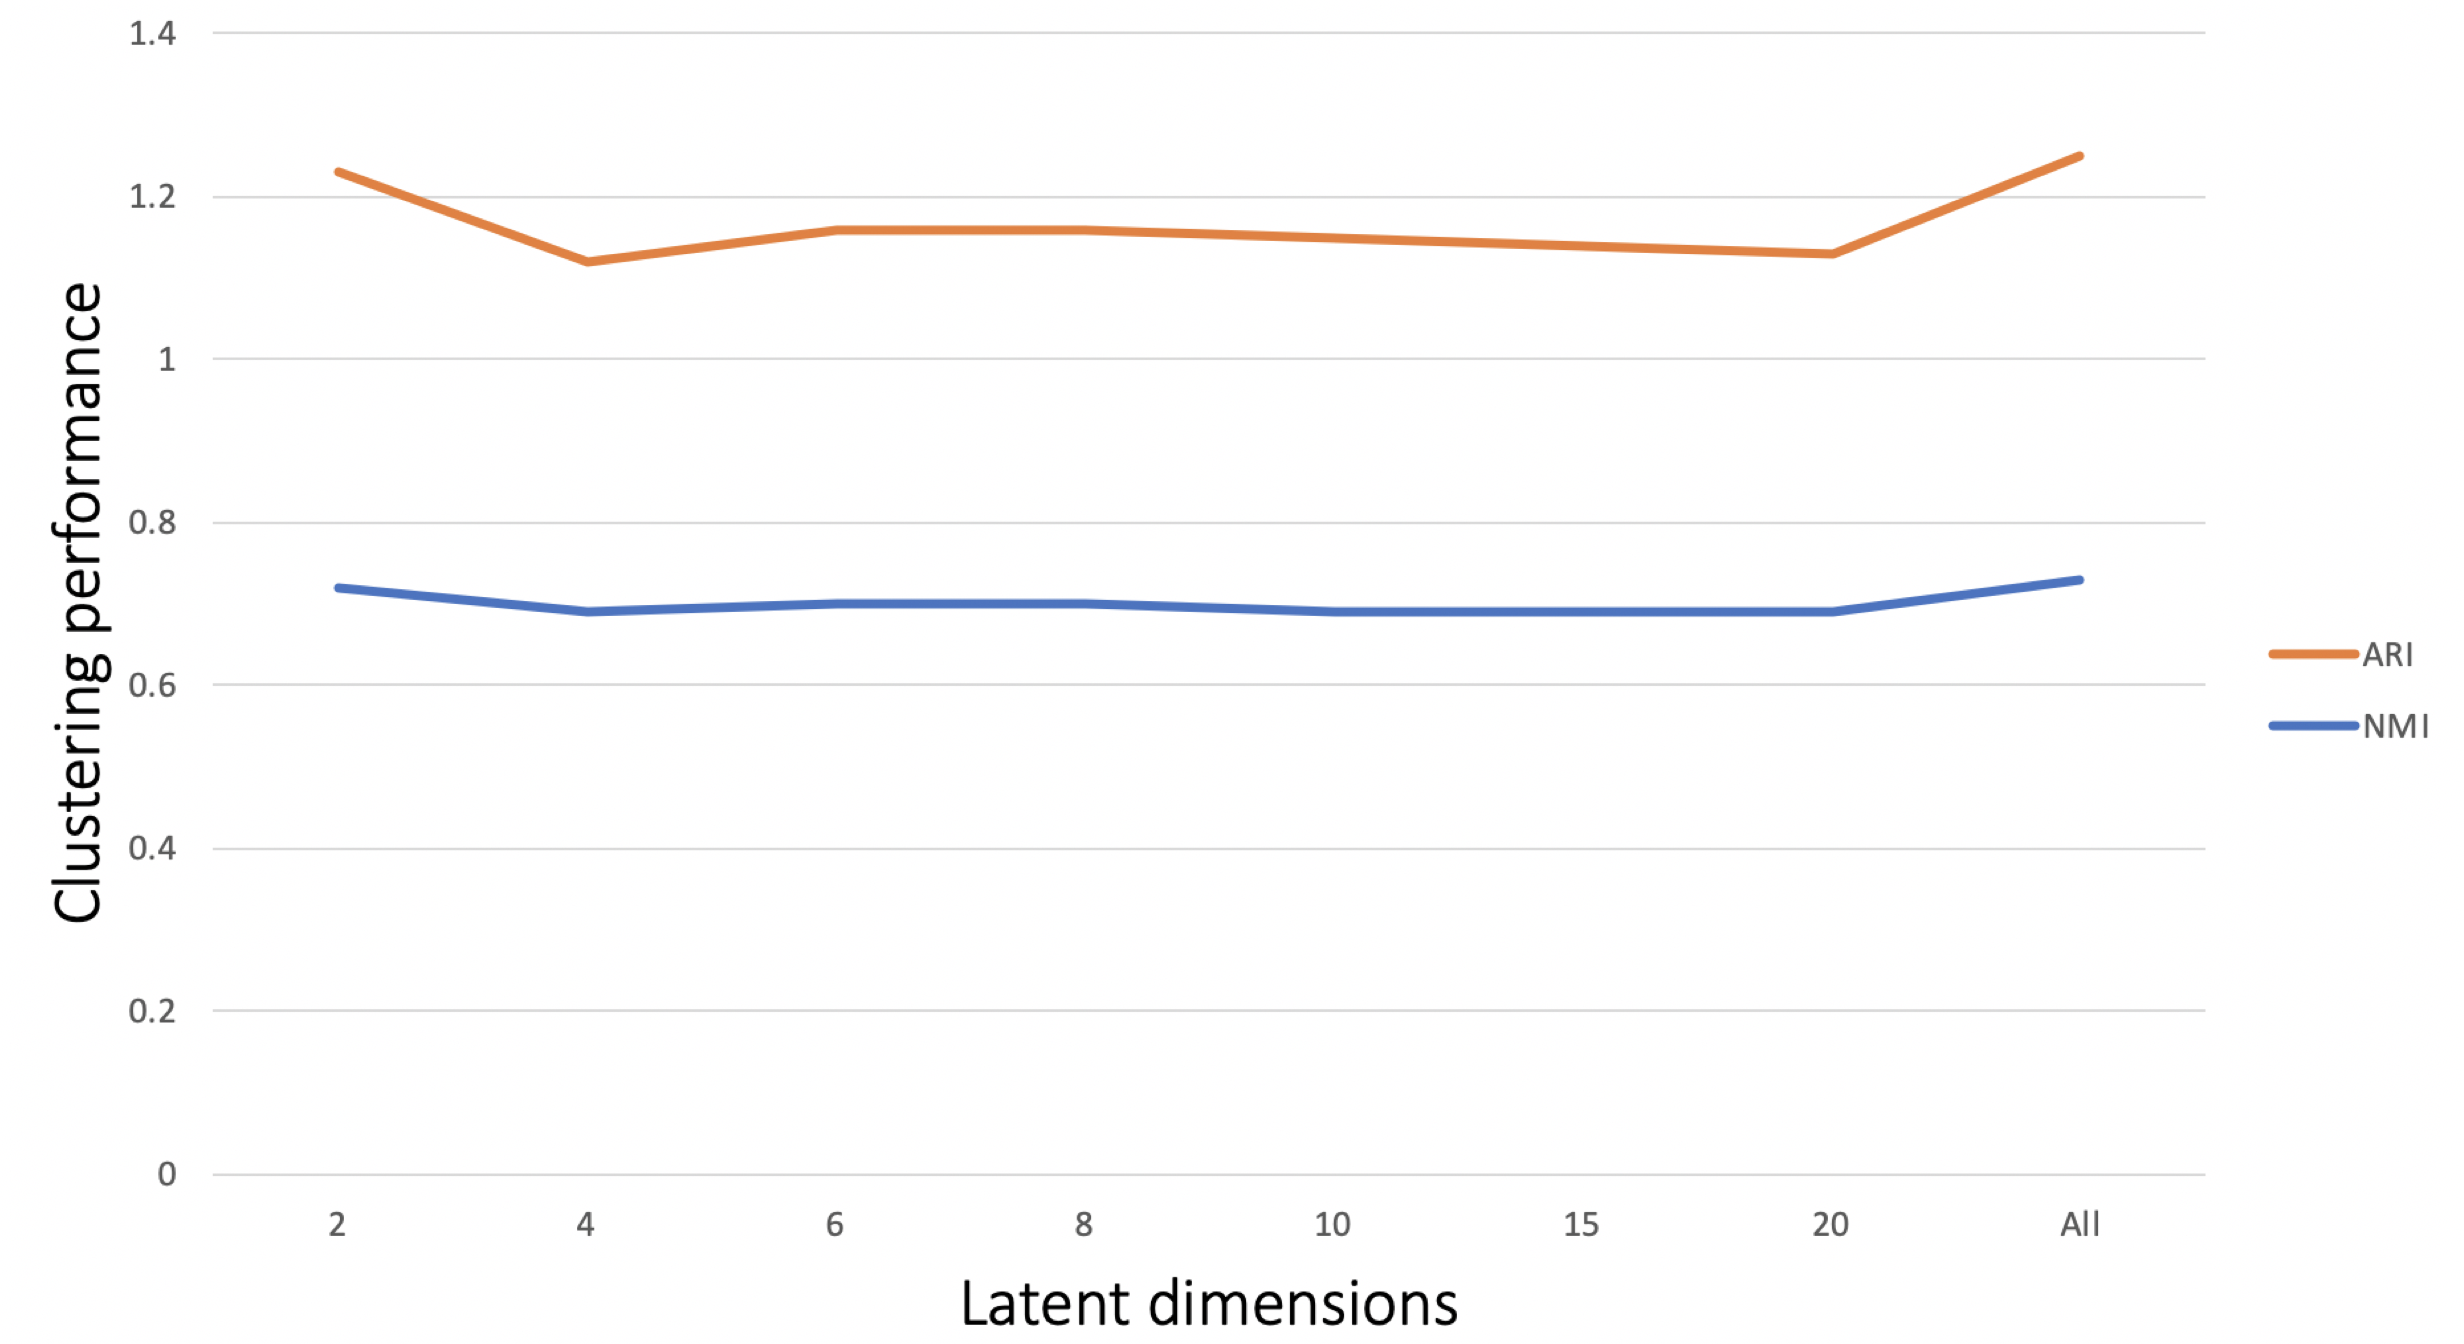
\includegraphics[width=0.8\textwidth]{figures/myfigures/dim.png}
    \caption{Clustering performance (NMI and ARI) of ZIVA under different latent dimensions.}
    \label{dim}
\end{figure}
